%!TEX root=../paper.tex

\section{Implementation}
Polite is implemented on top of Pharo Smalltalk and a context-sensitive extension of PetitParser is used to define its grammar using parsing expressions\cite{Kurs14a-ParsingContext}. The current implementation can be found online in the Zenodo data repository. The code examples from this paper are fragments of a larger example that can also be found in the Polite image available online \cite{kurs16-polite}. The image also contains a code editor that supports code highlighting as illustrated in Figure 1.

\begin{figure}[h]
	\centering
	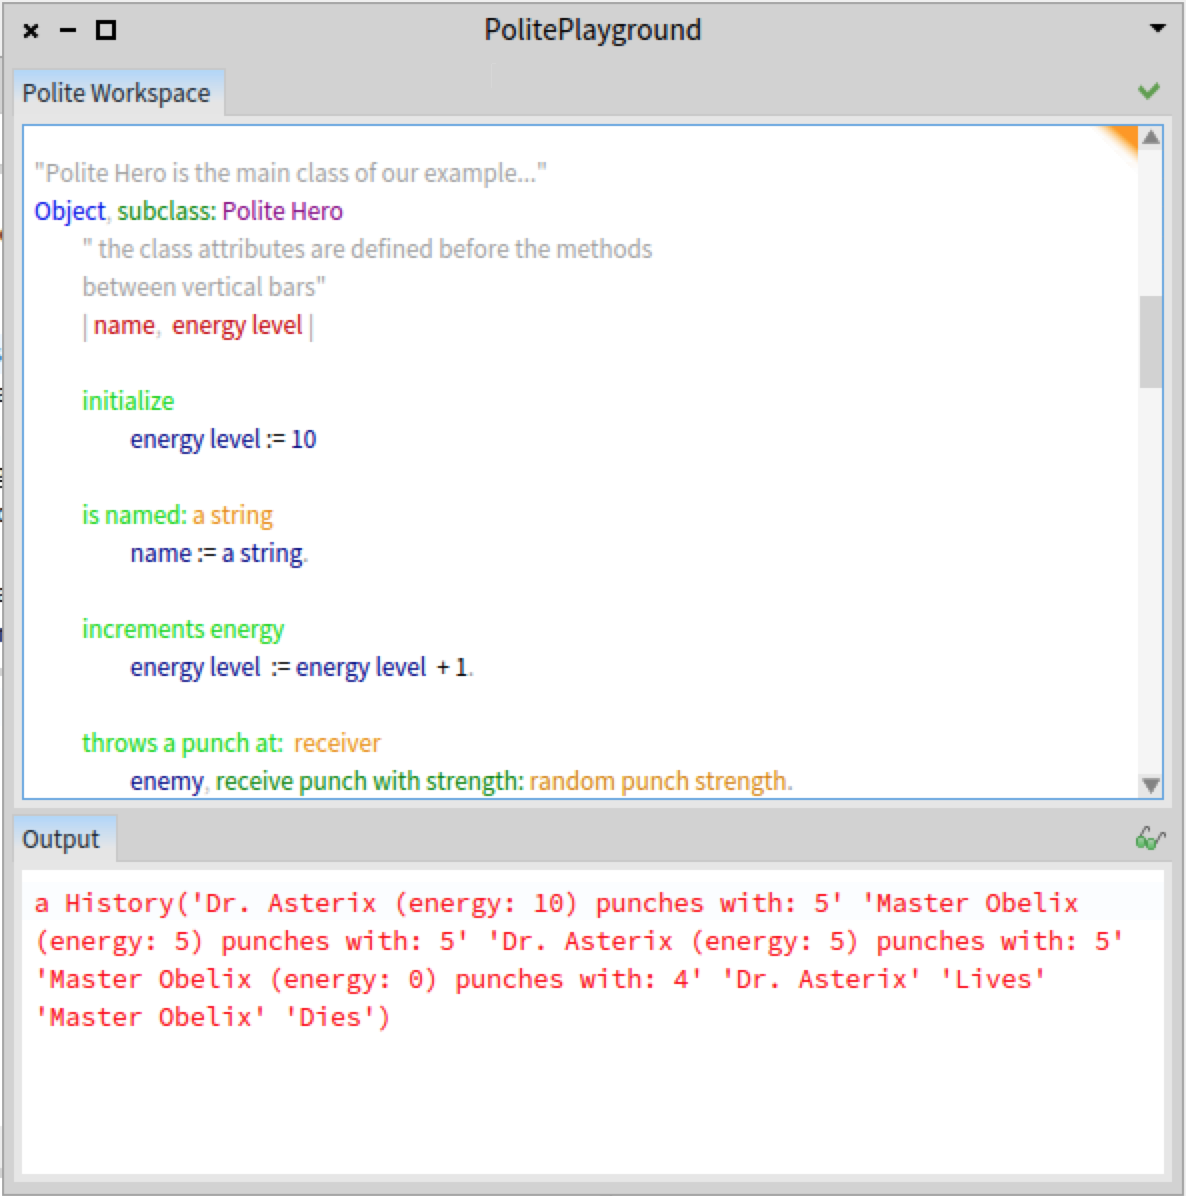
\includegraphics[width=0.45\textwidth]{images/playground.png}
	\caption{The Polite Playground provides a syntax highlighting code editor for Polite}
	\label{fig:figure1}
\end{figure}